%%%%%%%%%%%%%%%%%%%%%%%%%%%%%%%%%%%%%%%%%%%%%%%%%%%%%%%%%%%%%%%%%%%%%%%%
%    INSTITUTE OF PHYSICS PUBLISHING                                   %
%                                                                      %
%   `Preparing an article for publication in an Institute of Physics   %
%    Publishing journal using LaTeX'                                   %
%                                                                      %
%    LaTeX source code `ioplau2e.tex' used to generate `author         %
%    guidelines', the documentation explaining and demonstrating use   %
%    of the Institute of Physics Publishing LaTeX preprint files       %
%    `iopart.cls, iopart12.clo and iopart10.clo'.                      %
%                                                                      %
%    `ioplau2e.tex' itself uses LaTeX with `iopart.cls'                %
%                                                                      %
%%%%%%%%%%%%%%%%%%%%%%%%%%%%%%%%%%
%
%
% First we have a character check
%
% ! exclamation mark    " double quote  
% # hash                ` opening quote (grave)
% & ampersand           ' closing quote (acute)
% $ dollar              % percent       
% ( open parenthesis    ) close paren.  
% - hyphen              = equals sign
% | vertical bar        ~ tilde         
% @ at sign             _ underscore
% { open curly brace    } close curly   
% [ open square         ] close square bracket
% + plus sign           ; semi-colon    
% * asterisk            : colon
% < open angle bracket  > close angle   
% , comma               . full stop
% ? question mark       / forward slash 
% \ backslash           ^ circumflex
%
% ABCDEFGHIJKLMNOPQRSTUVWXYZ 
% abcdefghijklmnopqrstuvwxyz 
% 1234567890
%
%%%%%%%%%%%%%%%%%%%%%%%%%%%%%%%%%%%%%%%%%%%%%%%%%%%%%%%%%%%%%%%%%%%
%
\documentclass[12pt]{iopart}
%\newcommand{\gguide}{{\it Preparing graphics for IOP journals}}
%Uncomment next line if AMS fonts required
%\usepackage{iopams}  

\usepackage{subcaption}
\captionsetup{compatibility=false}
\usepackage{subfig}
\usepackage[pdftex]{graphicx}
\usepackage{epstopdf}
\graphicspath{{./images/}{./images/other_formats/}}
\DeclareGraphicsExtensions{.pdf,.png,.eps,.jpg}

%Place footnotes at the bottom of the page
\usepackage[bottom]{footmisc}

\begin{document}

\title[]{A Modular and Cost-Effective Superconducting Generator Design for Offshore Wind Turbines}
\footnote{Supported by MARINA}
\author{Ozan Keysan, Markus Mueller}

\address{Institute for Energy Systems,
University of Edinburgh, 
EH93JL, UK}
\ead{o.keysan@ed.ac.uk}

\begin{abstract}
For offshore wind energy, there is a trend  towards larger wind turbines. The increased power take-off system mass increases the installation cost of the turbine. Direct-drive superconducting generators have the potential to reduce the installation cost of wind turbines. For a successful entry to offshore wind energy market, a HTS generator should be as reliable as conventional generators. It is proposed that a stationary superconducting dc-field winding may increase the reliability of the generator. An axial-flux homopolar generator topology is proposed to be used in low-speed high-torque applications. The topology is modified by using two superconducting field windings to obtain a bipolar flux density distribution for higher power density. Different core types and dimensions were examined to find the most suitable design and a conceptual design of 6 MW, 12 rpm generator is presented.
\end{abstract}

%Uncomment for PACS numbers title message
%\pacs{00.00, 20.00, 42.10}
% Keywords required only for MST, PB, PMB, PM, JOA, JOB? 
%\vspace{2pc}
%\noindent{\it Keywords}: Article preparation, IOP journals
% Uncomment for Submitted to journal title message
%\submitto{\JPA}
% Comment out if separate title page not required
\maketitle

\section{Introduction}


Literatur:

In \cite{Chen2014}, a superconducting generator with stationary superconducting armature and field windings are shown, the machine is similar to a switched reluctance machine.

Cumleler madde madde degisecek

the average offshore wind turbine size is increasing to reduce the cost of energy.


There has been a remarkable increase in the installed renewable power capacity around the world for the last decade and this increase is expected to continue for many years \cite{Tong2010}. The onshore wind energy market is now quite mature, but there is a lot of ongoing research into offshore renewable energy devices which will benefit from higher wind speeds and higher capacity factors \cite{Tong2010}.  In offshore wind turbines, there is a trend towards higher power rated turbines to reduce installation and maintenance costs per kWh \cite{Bang2008}. According to market projections of \cite{offshore_wind_report2009}, annual world production of offshore wind turbines will continue to increase. Furthermore, the proportion of  the turbines rated over 5 MW will increase significantly for the next decade as seen from Fig. \ref{world_production}.

Currently, geared asynchronous machines hold a 70\% share of wind turbine generators \cite{Lesser2009}. Lesser \textit{et al.} compared costs of different generator types in \cite{Lesser2009}. They proposed that the aim of the offshore wind turbine industry is to manufacture 10 MW  turbines which cost \$ 2.7 M/MW or less. The current cost of wind turbines is about \$ 2 M/MW for onshore turbines and \$ 3.7 M/MW for offshore wind turbines with a typical rating of 2.5 MW for onshore and 3.6 MW for offshore \cite{Lesser2009}.

The feasible limit for an industrial 3-stage wind turbine gearbox is about 5 MW due to high torque requirements at very low speeds \cite{Lesser2009}. Moreover, gearboxes cause reliability issues in wind turbines. The reliability of wind turbine sub-assemblies have been compared in \cite{Spinato2009} using the data obtained from 6000 onshore wind turbines over 11 years. This study shows that, although the gearbox doesn't have the highest failure rate, the failures related to gearboxes result in the highest down-time periods (average 340 hours per failure). Note that, this data was obtained from onshore turbines; the downtime related to a gearbox failure for offshore turbines will be much higher, adding an extra cost of down-time on top of the maintenance cost. For example, the worst case scenario is a major failure at the beginning of the winter period and with no subsequent access to the turbine until the winter storms are gone \cite{Abrahamsen2010}.

There are some commercial solutions (mostly direct-drive permanent magnet generators) that aim to overcome this problem e.g. Harakosan, Vensys, Enercon. In \cite{Bang2008} different topologies for wind turbines have been compared. The highest power rated  commercial direct drive machine is the 4.5 MW, 13 rpm Enercon-E112 generator which has a 12 m diameter and 220 tonnes mass. The optimum weight for a 10 MW direct drive PM generator is greater than 300 metric tons including support structures with an air gap diameter greater than 10 meters \cite{Bang2008}. The installation cost of the turbine is directly related to the mass of the generator and nacelle. Moreover, the tower, the foundation and all other supporting structures have to be modified to carry the added mass of the generator. Considering the capability of current offshore installation vessels which is around 300 tonnes \cite{Lewis2007}, the demand for a high power density, low-speed direct-drive generator topology is clear.

One promising candidate to reduce the overall mass and volume of a large offshore wind turbine(up to 10 MW) power take-off system is High-Temperature Superconducting Generators (HTSG) \cite{Lesser2009, Lewis2007, Kalsi2004}. HTS machines can be scaled as fifth power of dimension in \cite{Kalsi2004} compared to third power for a conventional machine, which will become more dominant at direct-drive machines. It is stated in \cite{Lewis2007} that a 6 MW HTS direct drive generator may have 50 \% of the mass of a direct drive PM generator and the lower mass of generator may enable transport and installation of the turbine in one piece.


Data from direct-drive systems have been collected to compare mass to torque ratio of HTS machines with other type of generators. The result is presented in a bubble chart in Fig. \ref{generators_mass_comparison} and tabulated in Table \ref{generators_list}.  Note that, some of the machines are final designs or commercial products (e.g., Enercon, Harakosan), where some designs are provisional or it is not clear how the structural mass is estimated. Final designs tend to be heavier than initial designs, but it is believed that the graph will provide a good understanding of torque density capability of HTS machines.  The dashed line represents ratio of generator mass to torque for permanent-magnet machines which is estimated as 25 kg/kNm by Bang \textit{et al.} in \cite{Bang2008}. The Enercon-E112, which has a high $m/T$ ratio (66.6 kg/kNm) is the only copper field synchronous generator in the graph. The continuous line represents the linear trend line estimated using the HTS machines in the graph. The equation of the trend line is given in (\ref{mass_torque_eq}). It can be seen from the graph that HTS machines are generally lighter than PM generators for applications with torque requirements larger than 3000 kNm. There are two PMG topologies below the HTS machine trend line; a transversal flux permanent magnet machine \cite{Bang2009} and the NewGen topology which reduces the structural mass significantly \cite{Engstrom2004}. It should be noted that implementation of similar techniques to HTS machines can further decrease their mass. 

 \begin{equation}
     Mass(t)=0.011\times Torque(kNm)+45
     \label{mass_torque_eq}
 \end{equation}

\begin{figure}[t]
\centering
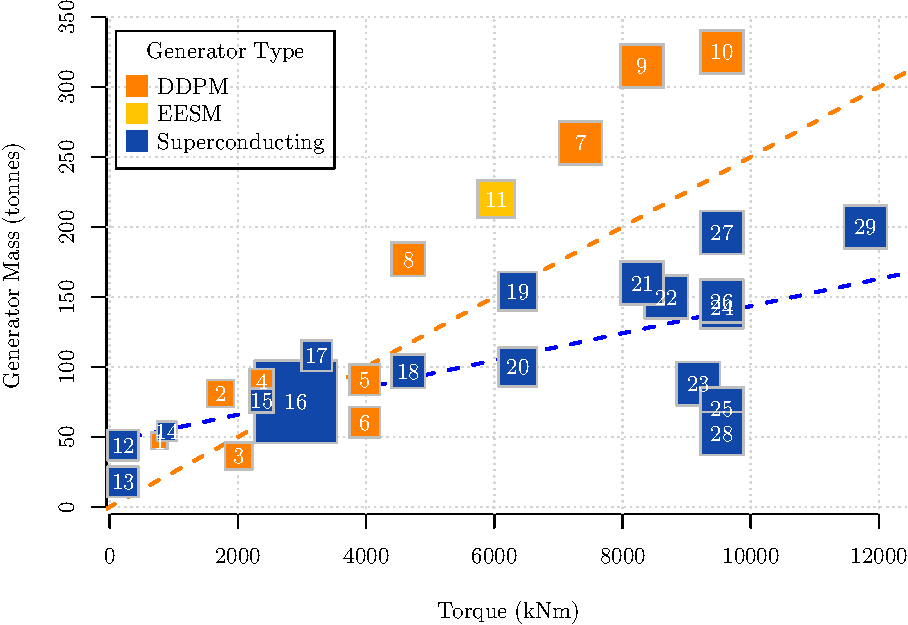
\includegraphics[]{generator_mass_compare}
\caption{Mass of different large direct-drive machines as a function of the torque, area of the square represents the power rating.
 DDPM: Direct drive permanent magnet generator, EESM: Electrically excited synchronous machine, Superconducting: High-temperature superconducting generator. Orange line represents generator mass to torque ratio ($m/T$) of 25 kg/kNm for permanent-magnet machines as given in \cite{Bang2008}. Blue line is the linear trend line for the superconducting machines.}
\label{generators_mass_comparison}
\end{figure}

 \subsection{Mass Comparison of Direct Drive Generators}
 \label{mass-comparison-section}

\begin{table}[]
\begin{minipage}{\textwidth}
\caption{Torque density comparison conventional and superconducting generators.}
\label{generators_list}
\centering
\begin{tabular}{llcccrrl}
\hline
 & Manufacturer & Power & Speed & Mass & Torque & Mass/T & Type \\
&  & (MW) & (rpm) & (t) & (kNm) & (kg/kNm) & \\
\hline
1 & Harakosan \cite{Duan2009}& 1.5 & 18 & 47.2 & 796 & 59.3 & PMG \\
2 & The Switch \cite{Duan2009} & 3.8 & 21 & 81 & 1728 & 46.9 & PMG  \\
3 & NewGen \cite{Engstrom2004} & 4 & 19 & 36.4 & 2010 & 18.1 & PMG  \\
4 & NREL-AMSC \cite{Maples2010}& 3.1 & 12.5 & 90 & 2368 & 38.0 & PMG\footnote{The machine is not optimised for minimum mass.}  \\ 
5 & Bang et. al. \cite{Bang2009} & 5 & 12 & 90.8 & 3979 & 22.8 & TFPM  \\
6 &  & 5 & 12 & 60.5 & 3979 & 15.2 & TFPM\footnote{Ring-shaped TFPM.}  \\
7 & NTNU Reference \cite{Smith2012} & 10 & 13 & 260 & 7346 & 35.4 & PMG \\
8 & NREL-AMSC \cite{Maples2010} & 6 & 12.3 & 177 & 4658 & 38.0 &  PMG\footnote{The machine is not optimised for minimum mass.} \\
9 &  & 10 & 11.5 & 315 & 8304 & 37.9 & PMG\footnote{The diameter is limited to 4.3 m.}  \\
10 & Bang et. al. \cite{Bang2008} & 10 & 10 & 325 & 9549 & 34.0 & PMG \footnote{Estimated mass.}  \\
11 & Enercon-E126 & 7.5 & 12 & 220 & 6031 & 36.4 & EESM \\
12 & Lee et. al. \cite{Lee2008} & 5 & 230 & 44 & 208 & 212.0 & HTSG\footnote{Homopolar superconducting machine.}  \\
13 &  & 5 & 230 & 18 & 208 & 86.7 &  HTSG\footnote{Air-cored superconducting synchronous machine.} \\
14 &  Maki \cite{Maki2008} & 2 & 21.5 & 54 & 888 & 60.8 & HTSG  \\
15 & NREL-AMSC \cite{Maples2010} & 3.1 & 12.5 & 76 & 2368 & 32.1 & HTSG  \\
16 & AMSC \cite{Kalsi2006} & 36.5 & 120 & 75 & 2905 & 25.8 & HTSG \\
17 & Maki \cite{Maki2008} & 5 & 14.8 & 108 & 3226 & 33.5 & HTSG \\
18 & NREL-AMSC \cite{Maples2010}  & 6 & 12.3 & 97 & 4658 & 20.8 & HTSG  \\
19 & Maki \cite{Maki2008}  & 8 & 12 & 154 & 6366 & 24.2 & HTSG  \\
20 & Converteam \cite{Lewis2007} & 8 & 12 & 100 & 6366 & 15.7 & HTSG  \\
21 & NREL-AMSC \cite{Maples2010} & 10 & 11.5 & 160 & 8303 & 19.3 & HTSG  \\
22 & AMSC \cite{Snitchler2010} & 10 & 11 & 150 & 8681 & 17.3 & HTSG  \\
23 & Abrahamsen et. al. \cite{Abrahamsen2010}& 10 & 10.4 & 88 & 9182 & 9.6 & HTSG \footnote{The machine is found to be economically infeasible.} \\
24 & General Electric \cite{Fair2012} & 10 & 10 & 143 & 9549 & 15.0 & HTSG \footnote{The generator actually uses NbTi low temperature superconductor wire.} \\
25 & AML \cite{Masson2011} & 10 & 10 & 70 & 9549 & 7.3 & HTSG \footnote{Fully superconducting generator with MgB2 wires.} \\
26 & Sung et. al. \cite{Sung2013} & 10 & 10 & 147 & 9549 & 15.4 & HTSG \footnote{With YBCO wire.} \\
27 & & 10 & 10 & 196 & 9549 & 20.5 & HTSG \footnote{With Bi-2223 wire.} \\
\hline
\end{tabular}
\end{minipage}
\end{table}

%Ustu ayni 
!!asagida tezden aynen alinan cumleler var rewrite

\section{Double Sided Claw Pole Concept}

In \cite{} a radial flux claw pole machine is presented. The novelty of the designs lays in having a single stationary superconducting field winding, which simplifies the cooling system. The rotor just consists of modular claw poles, which can be easily dissembled if required. The disadvantage of this machine is the unbalanced magnetic pull, which is proportional to the square of the air-gap magnetic flux density.

In the machine presented in this paper, the claw pole shape has been modified as shown in Figure~\ref{evolution_claw}. In this design, the rotor consists of a stationary superconducting field winding, two independent armature windings, and claw pole rotor.


\begin{figure}[]
  \centering
  \subfloat[Radial claw pole.]{\label{evolution_a}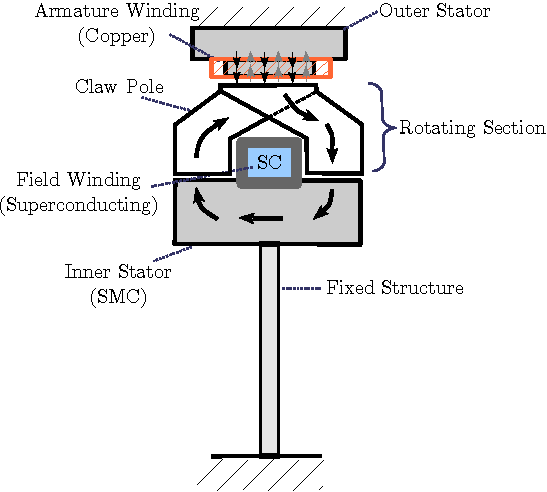
\includegraphics[scale=0.75]{radial_claw_pole}}
  \hspace{0.2in}
\subfloat[Axial claw pole.]{\label{evolution_b}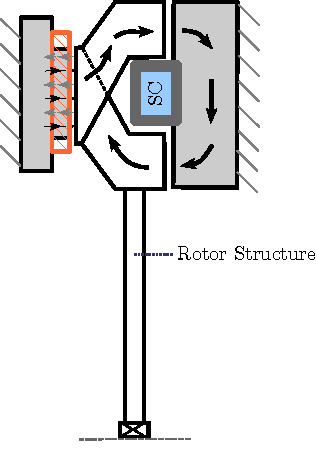
\includegraphics[scale=0.75]{axial_claw_pole}}
  
  \subfloat[Combined axial claw pole.]{\label{evolution_c}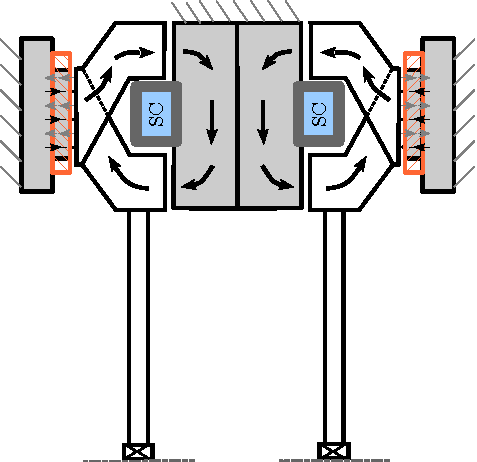
\includegraphics[scale=0.75]{double_axial_claw_pole}}
  \hspace{0.2in}
\subfloat[Double-sided claw pole.]{\label{evolution_d}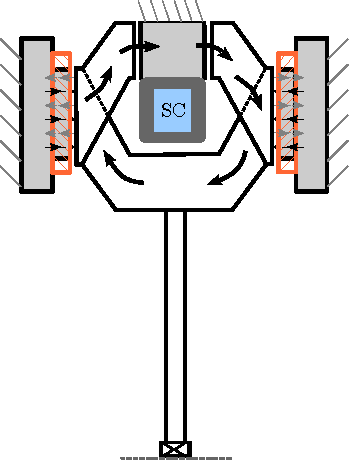
\includegraphics[scale=0.75]{double_claw_pole}}
    \caption{Evolution of the claw pole topology.} 
    \label{evolution_claw}
\end{figure}


The advantages of the double-sided claw pole topology can be listed as:

\begin{itemize}
  \item The machine has a stationary superconducting field winding, which means: no cryocoupler, no brushes or brushless exciters, no vibrational or rotational forces acting on the SC coil.
  \item The magnetic attraction forces on the rotor structure are symmetrical and cancel each other, which means reduced structural loads.
  \item The machine has two armature windings that can be operated independently. Thus, the modularity is increased.
  \item The machine uses significantly less superconducting coil due to iron-cored structure and loop-shaped field winding.
\end{itemize}

The 3D FEA model and the flux density vectors in the machine is presented in Figure~\ref{double_claw_parts}. From the figure it can be seen that the cores are saturated at 2.3 T. The flux density vectors shown in Figure~\ref{double_claw_B_vector_iso} verify the operation of the proposed topology as the magnetic flux created by the superconducting coil links both armature cores through the claw poles as depicted in Figure~\ref{evolution_d}.


\begin{figure}[]
  \centering
  \subfloat[Section of the machine.]{\label{double_claw_parts_iso}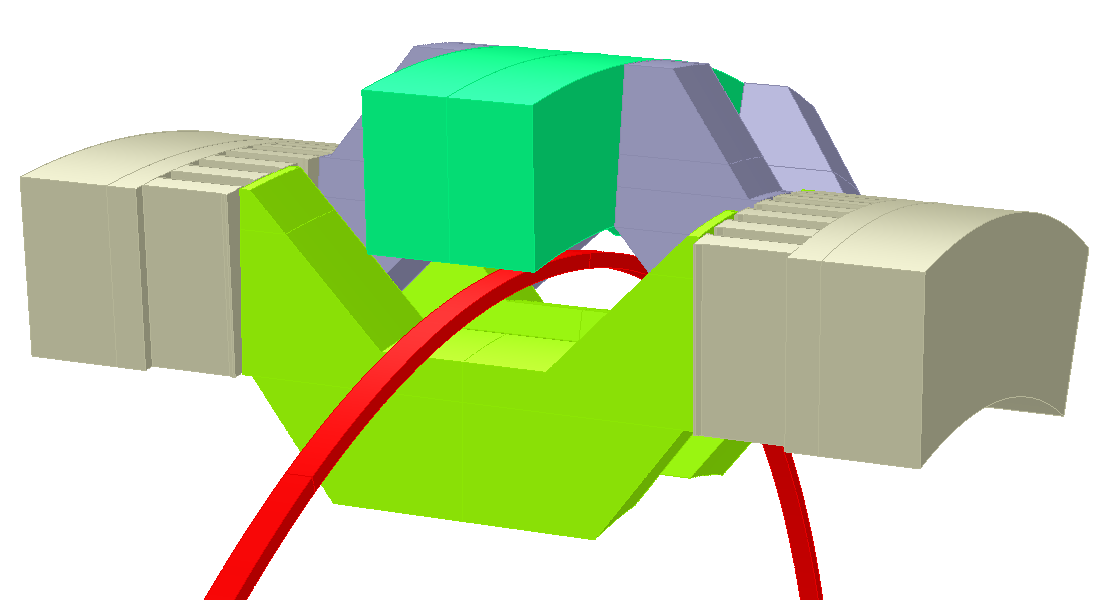
\includegraphics[scale=0.75]{double_claw_parts_iso}}
\hspace{0.5in}
\subfloat[Full machine.]{\label{double_claw_full}   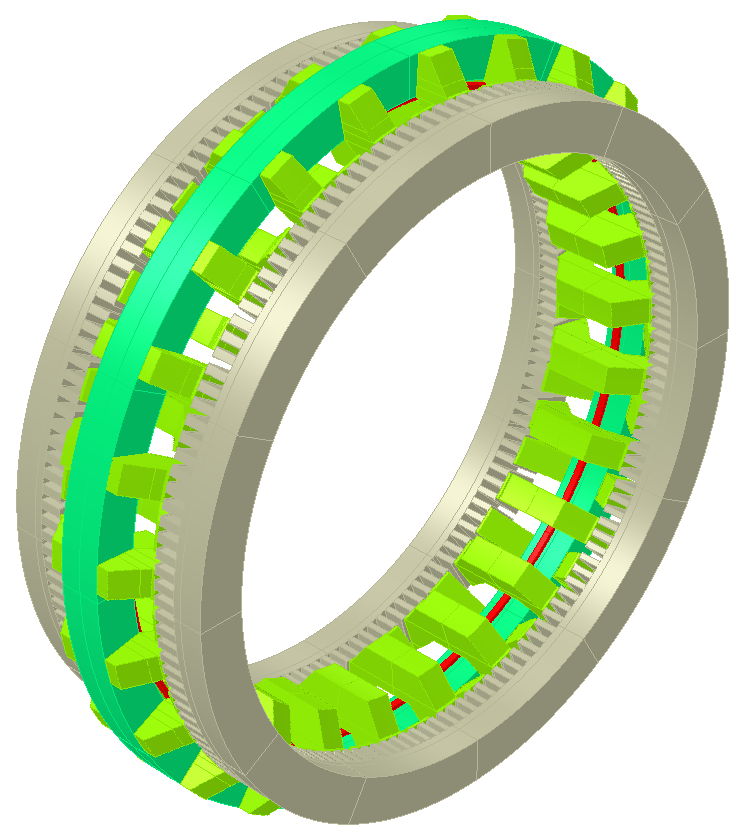
\includegraphics[scale=0.75]{double_claw_full}}

\subfloat[Flux density vectors.]{\label{double_claw_B_vector_iso}   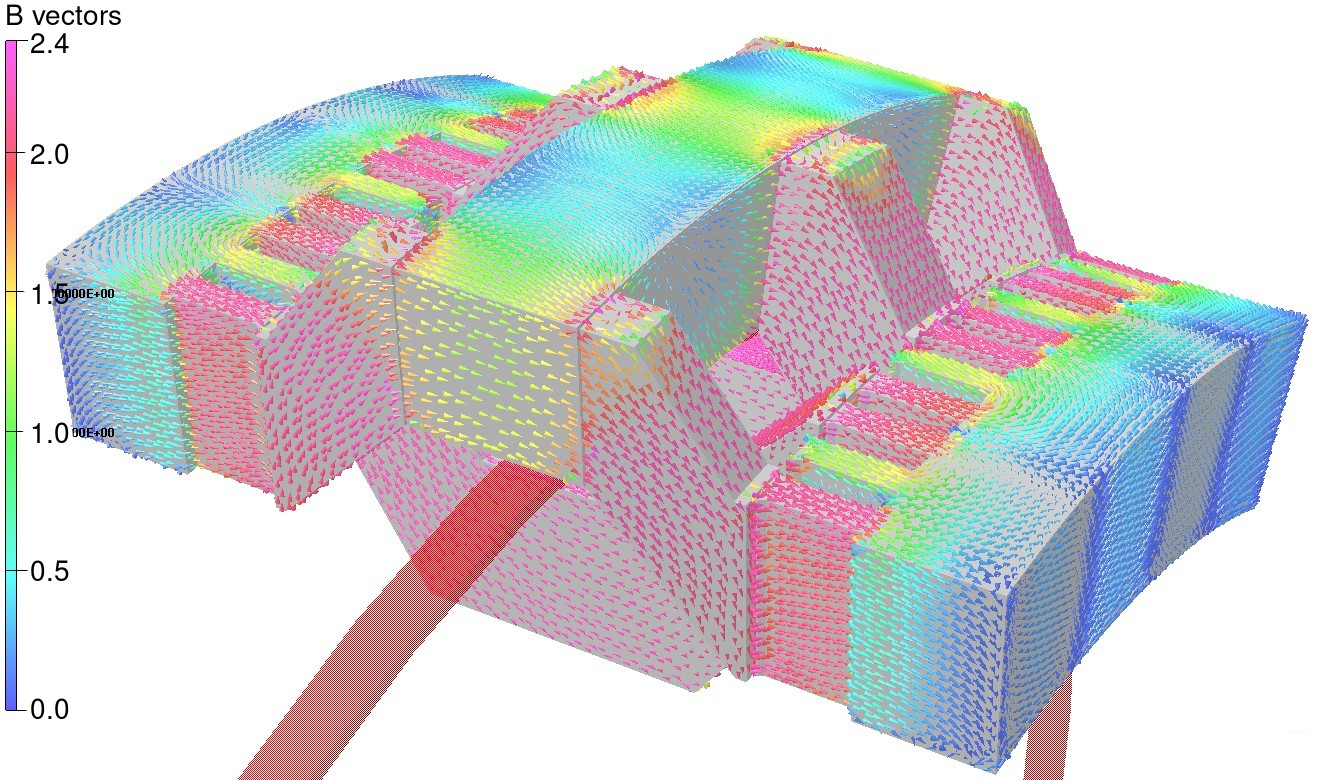
\includegraphics[scale=0.75]{double_claw_B_vector_iso}}

  \caption{The double-claw pole machine model and flux density vectors.} 
  \label{double_claw_parts}
\end{figure}

\subsection{Material Selection}

The proposed topology is iron-cored. Thus, the power density of the machine is limited by magnetic saturation , which makes the material selection very critical.  Vacuumschmelze introduced a cobalt-iron alloy called VacoFlux50, which  can be manufactured in laminations and has an impressive magnetic saturation limit with 2.35 T at 16 kA/m \cite{vacoflux}. This material is promising for superconducting machine designs with its high saturation limit.

% B-H characteristics of the VacoFlux50 is presented in \ref{vacoflux-bh}.
% \begin{figure}[]
%   \centering
%     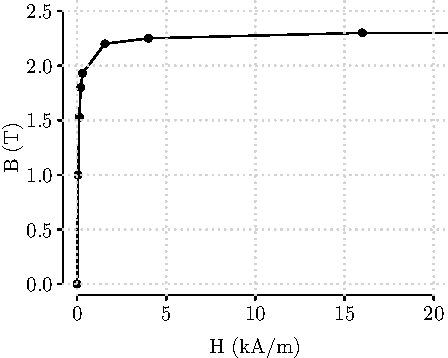
\includegraphics[]{vacoflux_50}
%   \caption{B-H curve for  VacoFlux50 cobalt-iron alloy\cite{vacoflux}.}
%   \label{vacoflux-bh}
% \end{figure}

\subsection{Sectioned Cryostat}

Although, the initial design is proposed with a single loop-shaped superconducting field winding, it is difficult to manufacture and install the field winding in MW scale. In the original design, the cryostat is fixed to the inner surface of the field core as shown in \ref{single_cryostat}. It is possible to mount another coil, which conducts current in the opposite direction, on the outer surface of the field core as in \ref{double_cryostat}. It is also possible to divide these cryostats in to two sections as shown in \ref{sectioned_cryostat}. In this way, it will be easier to manufacture and install the cryostat. Furthermore, now there are two independent cryostat, so in case of a failure the other cryostat can still operate until the maintenance. 


\begin{figure}[]
  \centering
  \subfloat[Single cryostat.]{\label{single_cryostat}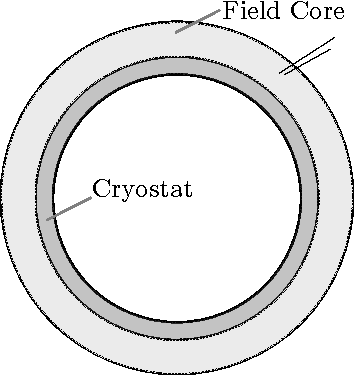
\includegraphics[scale=0.7]{single_cryostat}}  \hfill
  \subfloat[Double cryostat.]{\label{double_cryostat}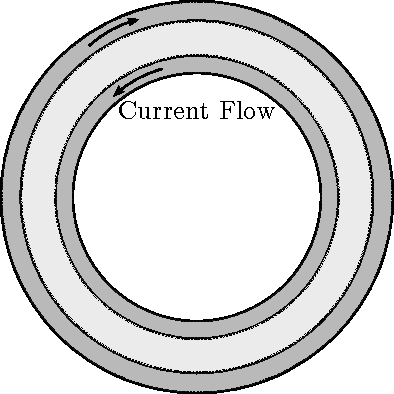
\includegraphics[scale=0.7]{double_cryostat}} \hfill 
  \subfloat[Sectioned cryostats.]{\label{sectioned_cryostat}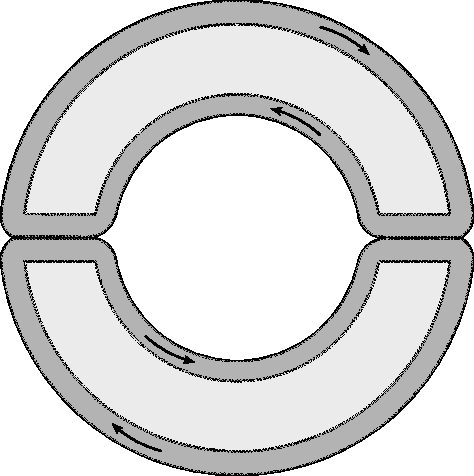
\includegraphics[scale=0.6]{sectioned_cryostat}}
    \caption{Sectioned cryostat design for the double-claw pole machine.} 
    \label{cryostat_variants}
\end{figure}


%The disadvantage is the total superconducting wire length is slightly increased due to  the intersection areas, which becomes less important at larger diameters. There is no field core where the two cryostats are adjacent, thus the flux density in the claw pole and the armature teeth will be lower, but this effect is ignored in the simulations. It is also possible to divide the armature core into the same number of sections to coincide with the field core. 

%The field core can also be fixed to a T-shaped core as presented in \ref{T_core}. In this configuration the cryostat and the superconducting coil is mounted to the field core as in \ref{T_core_solid}. The main difference in this configuration is two armature windings are now magnetically independent i.e. there are two separate flux loops in the machine. The flux lines cross the air-gap four times, thus the MMF requirements are reduced. However, the flux has to travel in the field core in a three-dimensional way, which requires SMC to be used. Furthermore, there are radial magnetic attraction forces acting on the large claw pole. Therefore, this configuration is not very suitable for large diameter machines, and the configuration presented in \ref{sectioned_cryostat} is used throughout this chapter.




\section{Design of a 10 MW Superconducting Generator}
 
As presented in the introduction section and in Table~\ref{generators_list}, 10~MW, 10~rpm superconducting generator designs are quite common in the literature, and a 10 MW double-sided claw pole machine design will be presented in this section.
\subsection{Electromagnetic Modelling}



\section{Optimization}




\subsection{Optimisation}

A parametrized model of the proposed topology is developed using Cobham-Opera \cite{Opera}. The parametrized model estimates the air gap flux density distribution, which is then used to estimate the power output of the machine.

The genetic algorithm optimization is realized using the genetic optimisation tool for R "rgenoud" \cite{Mebane2011}, which is an open-source tool with comprehensive optimisation methods and options and it can be easily modified to fit into any type of optimisation problem.


More details can be found on optimization algorithm in \cite{github-repo}


THe objective function is defined as the total active material mass. The boundaries of the problem is defined as follows:

degistir

\begin{itemize}
  \item  Outer Diameter: It is possible to reduce the active material mass by increasing the diameter. However, the outer diameter should be limited due to installation and manufacturing constraints.
  \item Power Output: The minimum power output required for the specific design.
  \item Phase Voltage: The minimum and the maximum phase voltage limits for connection to the power electronics and to the grid.
  \item Current Density: Maximum current density limit ensures that the temperature of the armature coils is within the acceptable range.
\end{itemize}


\section{Optimized 10 MW Design}

In this section, optimization results of a 10 MW, 10 rpm superconducting generator is presented. 

The inner radius limit is defined as 2.3 m. 

optimization output vs generation grafigi modifiye edilip verilebilir.

The main specifications of the optimum design is presented in \ref{10MW_design_parameters}.

dimension tanimlari yapilabilir

\begin{table}
  \centering
  \begin{tabular}{ll}
\hline
$R_{in}$ & 2288 mm \\
$N_{pole}$ & 88 \\
$h_{claw1}$ & 100 mm\\
$h_{claw}$ & 393 mm\\
$w_{claw}$ & 351 mm\\
$w_{core}$ & 393 mm\\
$w_{gap}$ & 121 mm\\
$h_{backcore}$ & 100 mm\\
$h_{w}$ & 172 mm\\
$k_{core-pole \, ratio}$ & 0.85 \\
\hline
 \end{tabular}
  \caption{Best design parameters for the 10 MW, 10 rpm design.}
  \label{10MW_design_parameters}
\end{table}

\begin{table}[t]
  \centering
  \begin{tabular}{ll}
\hline
Power Rating & 10 MW \\
Rotational Speed & 10 rpm \\
Number of Poles & 88 \\
\hline
Outer Diameter & 6.63 m \\
Armature Diameter & 5.84 m \\
Rotor Radius & 3.20 m \\
Inner Radius & 2.29 m \\
Axial Length & 1.38 m \\
\hline
Number of Stator Slots & 66 \\
Number of Turns & 96 \\
Induced Coil Voltage & 173 V$_{rms}$\\
Phase Voltage Voltage & 3.3 kV$_{ll}$ \\
\hline
 \end{tabular}
  \caption{Main specifications of the 10 MW, 10 rpm design.}
  \label{10MW_spec}
\end{table}


\ref{10MW_tooth_Bz} shows the flux density distribution in the stator tooth when the large claw pole and small claw pole are aligned with the middle stator tooth.
The total magnetic flux in the stator tooth versus rotor position is plotted in \ref{10MW_flux}.
The maximum flux in the stator tooth is 57.08 mWb when the large claw pole is aligned with the stator tooth. The flux waveform is not exactly symmetrical; the minimum flux is -53.66 mWb, 6 \% lower than the maximum flux value. This is mainly because of the geometrical difference between the large claw pole and the small claw pole and this difference can be minimised by shape optimisation or using different claw pole thickness. The induced voltage in a single coil at no load is plotted in \ref{10MW_voltage}, which has an electrical frequency of 7.33 Hz. There are 11 coils in series and two parallel branches for each phase. The main specifications of the machine are presented in \ref{10MW_spec}.

\begin{figure}[]
  \centering
  \begin{subfigure}{.4\columnwidth}
  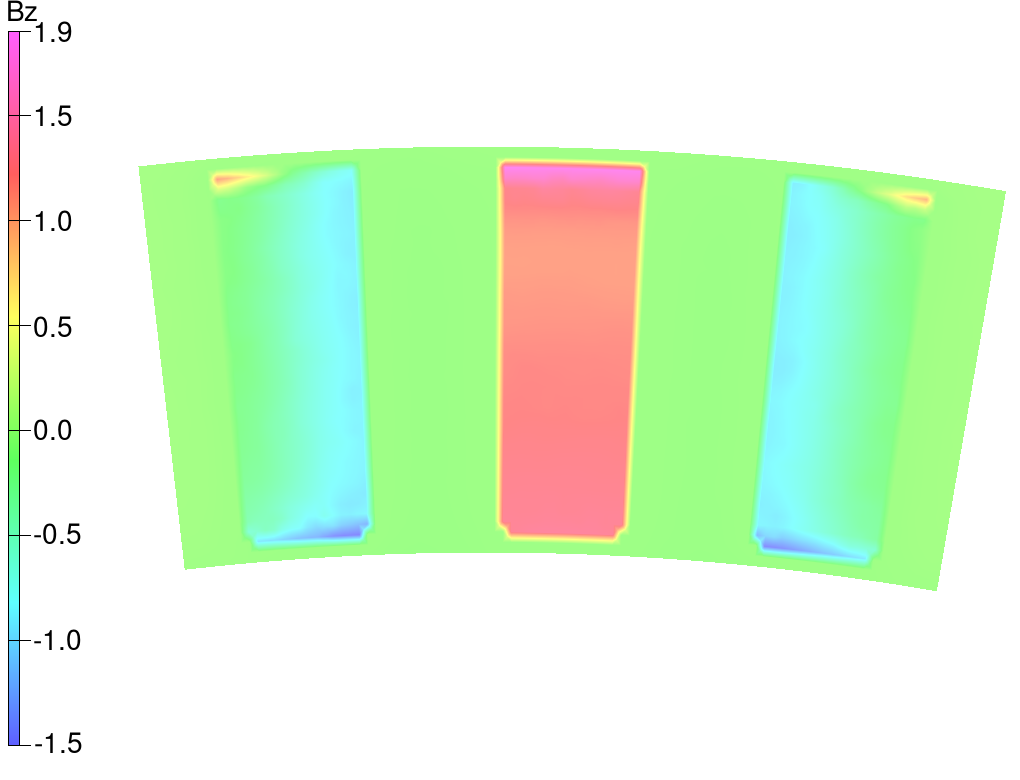
\includegraphics[]{Bz_0_deg}
  \caption{Middle tooth aligned with the large claw pole.}
  \label{Bz_0_deg}
  \end{subfigure}

  \begin{subfigure}{.4\columnwidth}
  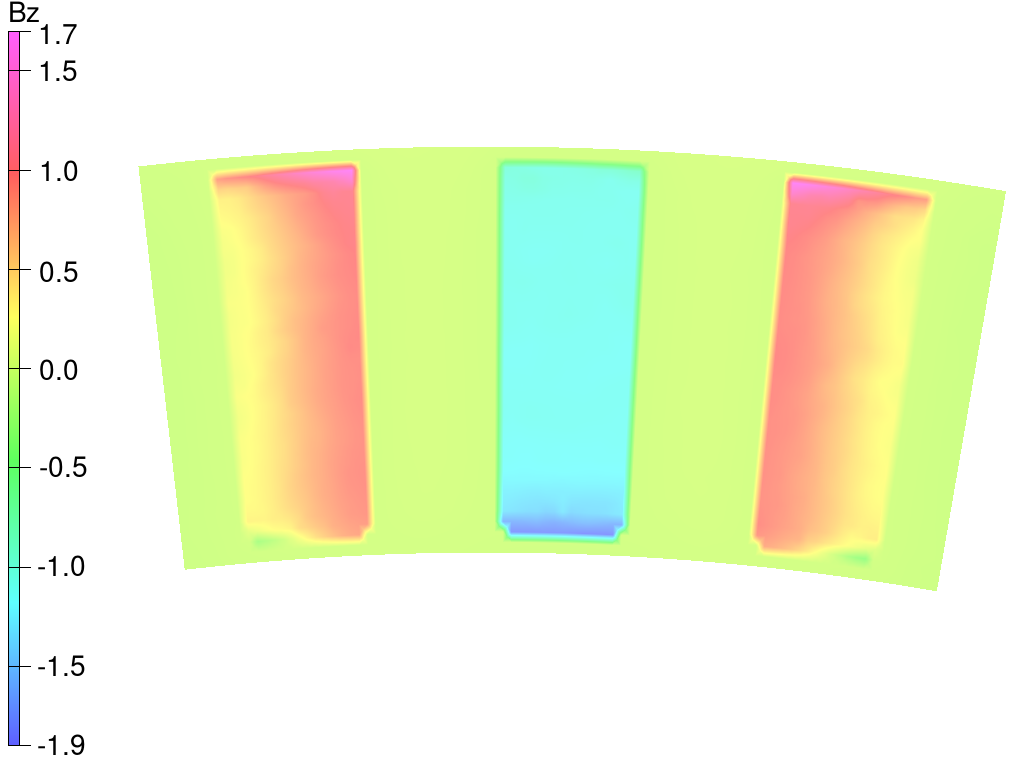
\includegraphics[]{Bz_90_deg}
  \caption{Middle tooth aligned with the small claw pole.}
  \label{Bz_90_deg}
  \end{subfigure}

  \caption{Flux density distribution in Z direction (into the page) in the stator teeth at mean coil radius.} 
  \label{10MW_tooth_Bz}
\end{figure}

\begin{figure}[t]
  \centering
    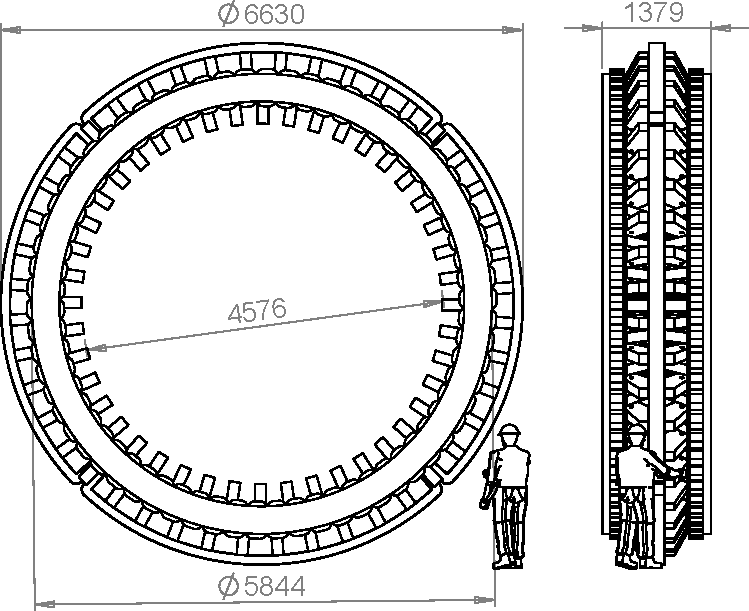
\includegraphics[]{10MW_outline_drawing}
  \caption{The outline dimensions of the 10 MW, 10 rpm generator design. Dimensions are in mm.}
  \label{10MW_drawing}
\end{figure}

The outline of the optimised generator is shown in \ref{10MW_drawing}. The machine has an outer diameter of 6.6 m and an axial length of 1.4 m, which is a similar size to a 5 MW direct-drive permanent magnet generator.
The active material mass in the rotor is about 24 tonnes. Stators on each side weight around 10 tonnes.

\begin{table}[t]
  \centering
  \begin{tabular}{lr}
\hline
Small Claw Pole & 114 kg \\
Large Claw Pole & 314 kg \\
Single Coil & 17.5 kg \\
Stator Core (Single Side) & 8,600 kg \\
Single Field Core Mass & 2,830 kg \\
\hline
Cryostat Mass & 1,200 kg \\
Cooling System Mass & 2,000 kg \\
%Number of Poles & 88 \\
%Total Copper Mass & 2,310 kg \\
Total Rotor Active Material & 23,850 kg \\
Stator (Single Side) & 9,755 kg \\
Total Field Core Mass & 11,320 kg \\
\hline
Total Active Material Mass & 57,9 tonnes \\
\hline
 \end{tabular}
  \caption{Mass estimations of the 10 MW, 10 rpm machine components.}
  \label{10MW_mass_spec}
\end{table}

The main losses in the machine are presented in \ref{10MW_efficiency}, which are dominated by the copper loss. 40 kW of air blowers are used for ventilation of armature coils. 
The electrical frequency of the machine is 7.3 Hz, which reduces the core losses in the machine. Furthermore, the core losses in the claw poles are negligible as the flux density magnitude and direction do not change. The core loss in the field core and stator core is calculated as 6.8 kW by extrapolating the core loss values presented in \cite{vacoflux}. The eddy current loss in the armature winding is neglected due to the low electrical frequency.


\begin{table}[t]
  \centering
  \begin{tabular}{lr}
\hline
%Input Power & 10,571 kW \\
%Pin=9987+510+7+24+30
Copper Loss & 510 kW \\
Core Loss & 7 kW \\
Cryocoolers & 24 kW \\
Air Blowers (Armature) & 40 kW \\
Output Power & 9,987 kW \\
\hline
Efficiency & 94.5 \% \\
%9987/10571
\hline
\end{tabular}
  \caption{Main losses and efficiency estimation for the 10 MW, 10 rpm design.}
  \label{10MW_efficiency}
\end{table}

\subsection{Estimation of the Heat Losses}

The 10 MW machine has four independent cryostats for increased modularity and ease of manufacturing. The mean length of the superconducting coil in each winding is 10.4 m. The magneto-motive-force of the superconducting coil is selected by the optimisation algorithm as 32.4 kAt. \ref{10MW_varying_MMF} shows the effect of varying MMF to the maximum stator tooth flux linkage. It can be seen from the figure that, the tooth saturates for MMF values higher than 32.4 kAt, and the choice of the GA is optimum.


\begin{figure}[t]
  \centering
    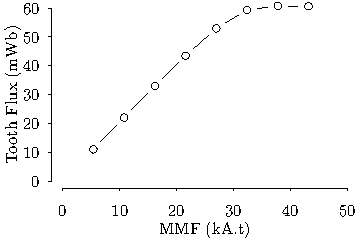
\includegraphics[]{10MW_varying_MMF}
  \caption{Stator tooth flux linkage variation with field winding MMF.}
  \label{10MW_varying_MMF}
\end{figure}

\begin{table}[t]
  \centering
  \begin{tabular}{ll}
\hline
Mean turn length & 10.4 m \\
MMF of the SC & 32.4 kAt \\
Number of Cryostats & 4 \\
Total SC requirement & 1348 kAt.m \\
\hline
 \end{tabular}
  \caption{Superconducting winding specifications for the 10 MW, 10 rpm design.}
  \label{10MW_hts_spec}
\end{table}
%Inner gap radius: 2681mm-2802mm
%Outer gap radius: 3195mm-3316mm
%Width=200mm, hgap=121mm 


\subsection{Superconducting Coil Requirements}

Tell about the air-gap difference in normal superconducting machines and the proposed one.

Including the flux penetrating into the superconducting coil, the critical current of MgB2 is assumed as 110 A, and 90 A is chosen as the safe operating current.

The field winding requires 32.4 kAt, which gives 360 turns. Assuming a fill factor of 0.75 and eight layers, the MgB2 wire can be wound on a 30x40~mm cross-section area. YBCO at the same temperature can conduct six times of its critical current at 77 K, which gives 504 A. 400 A is chosen as the safe operation current, which gives the number of turns as 81. Assuming a fill factor of 0.75 and three layers, the winding can fit in a 15x8 mm cross-section area.


The superconducting wire requirements for these three cases are presented in \ref{10MW_hts_wire_spec}. The superconducting wire requirement of the proposed machine is 15 km, which is much lower than for conventional superconducting machines. This is mainly because of the iron-cored structure and having a single superconducting winding instead of having separate superconducting coils for each pole.


\begin{table}[t]
  \centering
  \begin{tabular}{lccc}
& MgB2 & \multicolumn{2}{c}{YBCO} \\
\hline
Operating Temperature & 30 K & 30 K & 65 K \\
Current ($~0.8I_c$) & 90 A & 400 A & 100 A \\
Number of turns & 360 & 81 & 324 \\
Wire thickness & 0.67 mm & 0.22 mm & 0.22 mm \\
Wire width & 3.65 mm & 4.8 mm & 4.8 mm \\
Space & 30x40 mm & 15x8 mm & 15x32 mm \\
Wire length(per cryostat) & 3744 m & 842 m & 3370 m \\
Wire length (total) & 15.0 km & 3.4 km & 13.5 km \\
%Wire mass & 94 kg & 23 kg & 90 kg \\
\hline
 \end{tabular}
  \caption{Superconducting tape requirements for the 10 MW, 10 rpm design.}
  \label{10MW_hts_wire_spec}
\end{table}


\subsubsection{Cooling Power}

The main heat leakage elements in the cryostat can be listed as:

\begin{itemize}
  \item Gas heat conduction through the vacuum.
  \item Radiation heat from  warm walls of the cryostat.  \item Conduction through superconducting coil mechanical support.
  \item Heat leakage through current leads.
  %\item Eddy current loss.
\end{itemize}

These losses are estimated using a similar methodology presented in \cite{Abrahamsen2012, Simons2013}. As a worst case scenario, the operating temperature is assumed as 30 K.

detaylar verilebilir, Surface area ile ilgili olani goster.

\begin{table}
  \centering
  \begin{tabular}{lrr}
& 30 K & 65 K \\
& MgB2--90 A & YBCO--120 A \\
\hline
Gas Conduction (at $10^{-3}$ Pa) & 3.9 W & 3.4 W\\
Suspension Straps & 54.0 W & 50.0 W\\
Radiation & 17.5 W & 17.4 W\\
Current leads & 47.2 W & 48.8 W \\
Cold-head sleeve & 15.6 W & 15.6 W\\
Eddy Current & 4.0 W & 4.0 W\\
Other & 15.0 W & 15.0 W\\
\hline
Total loss & 157.2 W & 154.2 W\\
\hline
 \end{tabular}
  \caption{Thermal budget for the 10 MW, 10 rpm design. }
  \label{10MW_thermal_budget}
\end{table}

\begin{table}
  \centering
  \begin{tabular}{ll}
\hline
Cold head mass & 16.8 kg \\
Compressor mass & 176 kg \\
Flexible line mass & 4.2 kg \\
Total mass & 197 kg \\
Input power & 6 kW \\
\hline
 \end{tabular}
  \caption{Specifications of the Cryomech's AL230--CP950 cooling system (60~W @30~K) \cite{Cryomech2007}.}
  \label{cryocooler_spec}
\end{table}

To summarize, the proposed topology has the advantage of independent cryostats, which increases the modularity and overall reliability of the system. The total cryostat wall area is smaller compared to the conventional cylindrical cryostats, which helps to reduce the gas conduction and radiation losses. However, the sectioned cryostat results in higher number of current leads and suspension straps which increases the conduction losses. In general, the heat loss is within the reasonable values. For example in \cite{Snitchler2011}, it is stated that 6--10 CTI-1020 cryogenics are used for AMSC's 10 MW superconducting generator, which gives 280--450 W of cooling power.
In \cite{Stautner2012}, the total cooling requirement for the GE's 10 MW LTS superconducting generator is estimated as 131 W. In \cite{Abrahamsen2012}, 500~W is defined as the upper limit of the cooling power for a 5~MW superconducting generator.


\subsection{Structural Mass}
The excess structural mass in the large direct-drive generators is a serious issue. A very stiff structure is required to keep the air-gap clearance and the structural mass increases significantly with diameter (the mass of the torque arms is proportional to $R^3$ \cite{McDonald2008b}). The proposed machine has a smaller diameter than equivalent DDPM generators, which helps to reduce the structural mass. However, the high air-gap flux density increases the stress on the mechanical structure.

There are some studies trying to estimate the structural mass for DDPM generators \cite{McDonald2008b, Zavvos2012}. In \cite{Bang2010}, the structural mass of different DDPM generators are compared (see \ref{DDPM_structural_mass}). In \cite{Bang2010a} it is stated that the structural mass is around 55 \% of the mass of a 5 MW DDPM generator. In \cite{Zavvos2012}, the structural mass of a 10 MW DDPM generator with 7 m air-gap diameter is estimated as 248 tonnes. 

\begin{table}[t]
  \centering
  \begin{tabular}{lllcc}
 Power & Speed & Torque & Air-gap Diameter & Structural Mass\\ 
 \hline
2 MW & 19.5 rpm & 979 kNm & 4.3 m & 14.6 t \\
3 MW & 16 rpm & 1790 kNm & 5.1 m & 19.6 t \\
5 MW & 12.5 rpm & 3820 kNm & 6.1 m & 50.1 t \\
\hline
 \end{tabular}
  \caption{Structural mass estimation for different DDPM generators \cite{Bang2010}.}
  \label{DDPM_structural_mass}
\end{table}

There are only a few studies that consider the structural mass in a superconducting machine design. In \cite{Maples2010}, the mass of superconducting and permanent magnet machines are compared. In \cite{Sung2013}, the structural mass of a 10 MW, 10 rpm superconducting generator is estimated as 76 tonnes for a YBCO wire based generator, and 102 tonnes for a Bi-2223 wire based generator. The structural mass for these machines are around 50 \% of the overall mass.

Before proceeding into the structural mass estimation, it is useful to mention the different options to install the generator to the wind turbine nacelle. Firstly, an axial armature winding configuration with an inner rotor can be used as depicted in \ref{structure1}. In this configuration, the rotor structure is directly fixed to the turbine hub.  The stator structure supports both of the armature windings. The forces acting on the claw poles are balanced, however there is a net magnetic attraction force on each armature core, and the stator structure should be stiff enough to cope with these forces. An alternative to eliminate these axial forces is to rotate the claw poles as shown in \ref{structure2}. In this configuration, the forces on the armature core act radially and cancel each other along the circular symmetry. The disadvantage of this symmetry is that the stators are no longer identical (i.e. the inner stator has a smaller diameter, which causes flux density and the induced voltage characteristics to differ). Although, the machine can be designed to minimise this effect, this configuration is not covered in this study and an axial armature configuration is assumed.


In \cite{Zavvos2013}, the structural mass for different types of DDPM generators are optimised. Zavvos used FEA simulations and analytical models to estimate the deflection in the structure due to tangential and normal stresses. An analytical model is presented to estimate the structural mass of machines depending on the diameter, axial length and air-gap flux density. Although, the topology is quite different, the analytical model for transverse flux permanent magnet generators presented in \cite{Zavvos2013} is used to estimate the structural mass of the machine. The number of torque arms for stator and rotor is assumed to be 5, as it is found that it is the optimum value for minimum mass \cite{Zavvos2013}. The mass of the rotor structure and stator structure is presented along with the active material mass in \ref{10MW_total_mass}. Thus, the total mass of the generator is estimated as 184.2~t.


\begin{table}
  \centering
  \begin{tabular}{lr}
\hline
Rotor Structure & 42.8 t \\
Stator Structure & 83.5 t \\
\hline
Magnetic Core & 52.4 t\\
Copper & 2.3 t\\
Cooling - Cryostats & 3.2 t \\
\hline
Total Mass & 184.2 t \\
\hline
 \end{tabular}
  \caption{The structural and active material mass estimations for the 10 MW, 10 rpm machine.}
  \label{10MW_total_mass}
\end{table}

\begin{figure}[h!]
  \centering
  \begin{subfigure}{.4\columnwidth}
  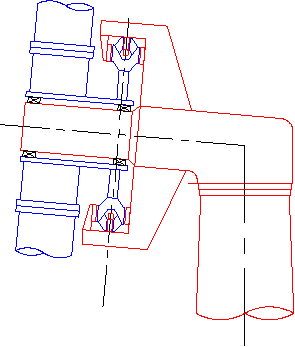
\includegraphics[scale=1.2]{structure_claw_radial_inner}
  \caption{Axial armature winding, inner rotor.}
  \label{structure1}
  \end{subfigure}
  \begin{subfigure}{.4\columnwidth}
  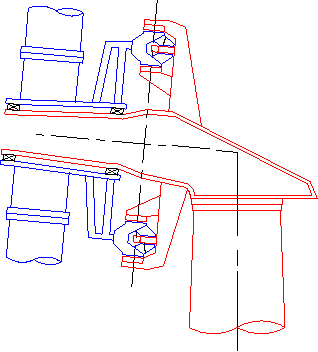
\includegraphics[scale=1.2]{structure_claw_axial}
  \caption{Radial armature winding.}
  \label{structure2}
  \end{subfigure}

  \caption{Two possible configurations for the installation of double-claw pole machine to a wind turbine (Drawings modified from \cite{Bang2010}).} 
  \label{DD_claw_pole_structures}
\end{figure}

\section{Mass Comparison}

It is now time to revisit \ref{generators_mass_comparison} of Chapter 1, which compares the torque densities of direct-drive permanent machines and superconducting machines. The 10 MW and 36.5 MW double-claw machine designs are placed in this graph in \ref{claw_pole_mass_compare}. The mass of the double-claw machines are above the trend-line of the superconducting machines (by 23 \% for the 10 MW machine, by the 36 \% for 36.5 MW machine).

The subcomponents masses (structure, magnetic core, copper and cooling) are also presented in the figure. The structural mass dominates the total mass in both designs (68 \% of the 10 MW design, 74 \% of the 36.5 MW design). The magnetic core employs 28 \% of the 10 MW design and 22 \% of the 36.5 MW design. The magnetic core mass could be reduced in air-cored type superconducting generators, but the structural mass would still be significant due to high magnetic attraction forces in the machine.

% \begin{figure}[ht]
%   \centering
%     \includegraphics[]{claw_pole_mass_bar_compare}
%   \caption{Mass comparison of the 10 MW and 36.5 MW double-claw machines with other direct-drive permanent magnet and  superconducting machines.}
%   \label{claw_pole_mass_compare}
% \end{figure}

\section{Conclusions}

In this chapter, a novel superconducting machine topology was presented, which is a modified version of the radial claw-pole design. In this concept, the forces acting on the rotor  are balanced, so it is easier to manufacture the machine at large diameters. There is no need for SMC material as all the magnetic core sections can be manufactured from electrical steel laminations. Furthermore, the amount of the field core mass is reduced, which results in a lighter design.

A major advantage of the double-claw pole topology is its modularity; instead of using a single large circular superconducting coil, it can be divided into smaller sections. The armature winding also has similar modularity due to concentrated coils. This has the following advantages:

\begin{itemize}
  \item Easier to manufacture and transport the machine.
  \item Independent operation of the cryostat sections.
  \item In the event of a fault in the cooling system or armature, the rest of the machine can be operated at part-load until maintenance.
  \item Faulty components can be replaced in situ.
\end{itemize}

All these factors are very beneficial for offshore wind turbines, where the maintenance and installation are difficult and expensive.

In order to find the optimum design, a parametrised FEA model was developed and coupled with a genetic algorithm optimisation tool. The tool was used to design a 10~MW, 10~rpm generator for wind turbines and a 36.5~MW, 120~rpm machine as a ship propulsion motor.

The 10 MW machine has an outer diameter of 6.6 m and an axial length of 1.4 m. The active material mass of the machine was calculated as 58 tonnes. Including the structure and the cooling system, the total mass is estimated as 184 tonnes. This is 23 \% higher than the trend-line of superconducting machines, but still 40 \% lighter than the similar rated direct-drive permanent magnet generators.
%10 MW, 300t
Structural mass is a significant component of total mass (around 70 \%). In fact, it is expected that it will be similar for all superconducting machines due to high airgap flux densities, although, the structural mass is usually neglected in direct-drive superconducting machine designs. Further improvements can be made by developing novel structures, and coupling the optimisation with structural design.

One of the most important advantages of the proposed topology is the low superconducting wire requirement compared to other superconducting machine designs. For example, 10 MW air-cored superconducting generators require more than 500 km of superconducting wire (see \ref{sec:hts-wind}). Other machines require around 100 km of superconducting wire. However, the proposed 10 MW double-claw machine requires just 15 km MgB2 tape at 30 K or 13.5 km YBCO tape at 65 K. The electrical power required for cooling is estimated as 24 kW (just 0.24 \% of the total power rating). 


To conclude, it has been shown that, the claw pole topology can be applied as a direct-drive generator (and ship propulsion motor). In terms of mass, it may not be as competitive as other superconducting machine designs, but it has clear advantages in terms of modularity and increased reliability. Furthermore, it uses much less superconducting wire and is expected to be more cost-competitive than other superconducting generator designs.

\bibliography{references}
\bibliographystyle{IEEEtran}



\section*{References}
\begin{thebibliography}{10}
\bibitem{book1} Goosens M, Rahtz S and Mittelbach F 1997 {\it The \LaTeX\ Graphics Companion\/} 
(Reading, MA: Addison-Wesley)
\bibitem{eps} Reckdahl K 1997 {\it Using Imported Graphics in \LaTeX\ } (search CTAN for the file `epslatex.pdf')
\end{thebibliography}

\end{document}

